


\documentclass{article}

\usepackage[romanian]{babel}
\usepackage{graphicx}
\usepackage{hyperref}
\usepackage{tikz}
\usepackage{pgfplots}




\author{Eduard-Mihail Hamza}
\title{Comparație experimentală între un Algoritm Genetic și varianta sa optimizată prin coduri Gray și Hill Climbing pentru minimizarea unor funcții cu număr variabil de parametri}

\begin{document}
\maketitle

\section{Introducere}

În analiza matematică, maximul și minimul unei funcții sunt cele mai mari, respectiv cele mai mici valori, pe care funcția le poate lua, fie pe un anume interval (caz în care poartă denumirea de maxim/minim local) sau pe întreg domeniul de definiție al funcției (caz în care se numește maxim/minim global).\\ \\
În acest raport se va realiza o comparație între un \textbf{algoritm genetic de minimizare} și \textbf{varianta sa optimizată} cu coduri Gray și Hill Climbing și se vor prezenta câteva date experimentale ce caracterizază execuția acestor algoritmi de aflare a minimului global al unei funcții cu număr variabil de parametri.

 
\subsection{Motivație}
Problemele de optimizare a unei funcții presupun gasirea minimului sau maximului unei funcții pe un interval. Astfel de probleme se abordează de obicei, atunci când instrumentele matematice clasice nu mai pot oferii soluții, cu ajutorul algoritmilor genetici. Una dintre cele mai mari provocări ale acestor algoritmi de optimizare este găsirea minimului/maximului global fără a rămâne blocați in minime/maxime locale.\\
Acest raport își propune să observe care dintre cele 2 metode amintite mai sus are rezultate mai bune în funcție de fiecare funcție de test în parte și în funcție de dimensiunea fiecărei funcții.

\section{Metode}
Implementarea \textbf{algoritmului genetic inițial} s-a realizat dupa o schmeă clasică în care se generează o populație inițială care apoi evoluează de lungul mai multor generații (prin crossovere și mutații) sub controlul unei funcții fitness care măsoară meritul individual.\\
Mai jos sunt amintite câteva detalii de implementare:
\begin{itemize}
\item Număr generații: $1000$
\item Probabilitate mutație: $0.001$
\item Probabilitate crossover: $0.4$
\item Monstră statistică: $30$
\end{itemize}
În ceea ce privește metoda de selecție a fost folosită \textbf{roata norocului}, metodă prin care numărul estimat de copii pe care îl primește un individ este proporțional cu fitness-ul său împărțit la fitness-ul total al populației.\\ \\
Mai jos este prezentat codul \textbf{funcței fitness} folosită: 
\begin{verbatim}
def fitness(individ, fct):
    global dimension

    Epsilon = 0.1
    result = fct(decode(individ))

    if fct == Schwefel:
        result = result + 418.9829 * dimension

    if fct == Michalewicz:
        result = -1 * result

    fitness_value = 1 / (result + Epsilon)

    return fitness_value
    
    
\end{verbatim}
Pentru \textbf{varianta optimizată} s-a folosit algoritmul genetic inițial, dar reprezentarea soluțiilor a fost realizată folosind \textbf{codificare Gray}, iar pe fiecare best găsit de-a lungul generațiilor s-a aplicat un \textbf{Hill Climbing} (cu stopping condition micșorat la $t < 50$). De asemenea, probabilitatea de mutație a fost redusă la 0.01.\\
În cazul primului algoritm pentru \textbf{reprezentarea soluțiilor} s-au folosit șiruri de biti, iar \textbf{precizia} utilizată a fost $10^{-2}$ (2 zecimale).
\clearpage
\section{Experiment}
Pentru testarea algoritmilor vom folosi următoarele funcții:
\begin{enumerate}
\item \textbf{Functia lui De Jong 1}
$$ f(x) = \sum_{i=1}^n x_i^2, 
x_i \in \left[ -5.12, 5.12 \right]$$

\includegraphics[scale=0.4]{spheref.png}

Minim global: 0

\item \textbf{Functia lui Schwefel}
$$ f(x) = \sum_{i=1}^n -x_i \cdot \sin (\sqrt{\mid x_i\mid}),
x_i \in \left[ -500, 500\right]  $$

\includegraphics[scale=0.4]{schwef.png}

Minim global: $-n \cdot 418.9829$
\item \textbf{Functia lui Rastrigin}
$$ f(x) = A \cdot n + \sum_{i=1}^n \left[ x_i^2 - A \cdot cos(2 \pi x_i) \right],
A = 10, x_i \in \left[ -5.12, 5.15 \right]$$

\includegraphics[scale=0.4]{rastr.png}

Minim global: 0
\item \textbf{Functia lui Michalewicz}
$$ f(x) = -\sum_{i=1}^n \sin (x_i) \cdot \left( \sin \left( \frac{i \cdot x_i^{2}}{\pi} \right) \right)  ^{2m},
m = 10, x_i \in \left[ 0, \pi \right] $$

\includegraphics[scale=0.4]{michal.png}

Minim global: -4.687 (n=5), -9.66 (n=10)
\end{enumerate}


\section{Rezultate}
teoretic = minimul teoretic al funcției (cel corect)\\\
minim = cel mai bun minim returnat de algoritm\\
medie = media minimelor obținute\\
$\sigma$ = deviație standard\\
timp = timpul mediu de execuție în secunde\\
GA = algoritm genetic\\
GA opt = varianta optimizată a algoritmului genetic\\
BIHC = Best Improvment Hill Climbing\\
FIHC = First Improvment Hill Climbing\\
SA = Simulated Annealing


\subsection{5 dimensiuni}

\begin{figure}[!h]
\begin{tabular}{||c|||l|l|l|l||}
  \hline
  \multicolumn{5}{||c||}{Rastrigin (teoretic min=0)} \\ \hline
  Algoritm & minim & medie & $\sigma$ & timp(s) \\ \hline \hline
  GA & 0.02 & 2.80 & 1.65 & 8.273 \\ \hline
  GA opt& 1.01 & 1.77 & 0.60 & 13.927 \\ \hline
  BIHC & 0.02 & 1.53 & 0.72 & 2.474\\ \hline
  FIHC & 0.02 & 2.04 & 1.25 & 0.475 \\ \hline
  SA & 1.01 & 6.12 & 3.49 & 0.527 \\ \hline
\end{tabular}
\caption{Rastrigin 5 dimensiuni - monstră statistică 30} 
\end{figure}

\begin{figure}[!h]
\begin{tabular}{||c|||l|l|l|l||}
  \hline
  \multicolumn{5}{||c||}{DeJong1 (teoretic min=0)} \\ \hline
  Algoritm & minim & medie & $\sigma$ & timp(s) \\ \hline \hline
  GA & 0.00 & 0.00 & 6.81 & 7.953 \\ \hline
  GA opt & 0.00 & 0.00 & 0.00 & 11.22 \\ \hline
  BIHC & 0.00 & 0.00 & 0.00 & 3.612\\ \hline
  FIHC & 0.00 & 0.00 & 0.00 & 0.469 \\ \hline
  SA & 0.00 & 0.00 & 0.00 & 0.505 \\ \hline
\end{tabular}
\caption{DeJong1 5 dimensiuni - monstră statistică 30} 
\end{figure}
\clearpage
\begin{figure}[!h]
\begin{tabular}{||c|||l|l|l|l||}
  \hline
  \multicolumn{5}{||c||}{Michalewicz (teoretic min=-4.687)} \\ \hline
  Algoritm & minim & medie & $\sigma$ & timp(s) \\ \hline \hline
  GA & -2.34 & -1.88 & 0.26 & 7.817 \\ \hline
  GA opt & -3.64 & -2.97 & 0.49 & 9.927 \\ \hline
  BIHC & -3.69 & -3.69 & 0.00 & 1.868\\ \hline
  FIHC & -3.69 & -3.68 & 0.01 & 0.377 \\ \hline
  SA & -3.69 & -3.53 & 0.13 & 0.46 \\ \hline
\end{tabular}
\caption{Michalewicz 5 dimensiuni - monstră statistică 30} 
\end{figure}

\begin{figure}[!h]
\begin{tabular}{||c|||l|l|l|l||}
  \hline
  \multicolumn{5}{||c||}{Schwefel (teoretic min=-2094.91)} \\ \hline
  Algoritm & minim & medie & $\sigma$ & timp(s) \\ \hline \hline
  GA & -2094.91 & -1990.00 & 90.00 & 12.321\\ \hline
  GA opt & -1913.46 & -1706.49 & 142.13 & 185.15 \\ \hline
  BIHC & -2094.80 & -2068.71 & 36.52 & 14.522\\ \hline
  FIHC & -2094.59 & -2020.11 & 39.16 & 1.691 \\ \hline
  SA & -2094.79 & -1926.10 & 120.03 & 1.43 \\ \hline
\end{tabular}
\caption{Schwefel 5 dimensiuni - monstră statistică 30} 
\end{figure}

\subsection{10 dimensiuni}


\begin{figure}[!h]
\begin{tabular}{||c|||l|l|l|l||}
  \hline
  \multicolumn{5}{||c||}{Rastrigin (teoretic min=0)} \\ \hline
  Algoritm & minim & medie & $\sigma$ & timp(s) \\ \hline \hline
  GA & 3.10 & 11.34 & 4.22 & 15.267 \\ \hline
  GA opt & 6.98 & 10.76 & 1.94 & 24.301 \\ \hline
  BIHC & 3.31 & 6.23 & 1.67 & 18.516\\ \hline
  FIHC & 5.59 & 9.66 & 2.29 & 2.089 \\ \hline
  SA & 5.59 & 14.07 & 4.60 & 2.07 \\ \hline
\end{tabular}
\caption{Rastrigin 10 dimensiuni - monstră statistică 30} 
\end{figure}

\begin{figure}[!h]
\begin{tabular}{||c|||l|l|l|l||}
  \hline
  \multicolumn{5}{||c||}{DeJong1 (teoretic min=0)} \\ \hline
  Algoritm & minim & medie & $\sigma$ & timp(s) \\ \hline \hline
  GA & 0.00 & 0.00 & 0.00 & 14.736 \\ \hline
  GA opt & 0.00 & 0.00 & 0.00 & 24.058 \\ \hline
  BIHC & 0.00 & 0.00 & 0.00 & 27.31\\ \hline
  FIHC & 0.00 & 0.00 & 0.00 & 2.004 \\ \hline
  SA & 0.01 & 0.02 & 0.00 & 1.984 \\ \hline
\end{tabular}
\caption{DeJong1 10 dimensiuni - monstră statistică 30} 
\end{figure}

\begin{figure}[!h]
\begin{tabular}{||c|||l|l|l|l||}
  \hline
  \multicolumn{5}{||c||}{Michalewicz (teoretic min=-9.66)} \\ \hline
  Algoritm & minim & medie & $\sigma$ & timp(s) \\ \hline \hline
  GA & -3.90 & -3.00 & 0.40 & 14.466 \\ \hline
  GA opt & -6.32 & -4.34 & 1.07 & 18.819 \\ \hline
  BIHC & -8.48 & -8.22 & 0.14 & 13.855\\ \hline
  FIHC & -8.45 & -8.00 & 0.20 & 1.653 \\ \hline
  SA & -8.45 & -7.90 & 0.31 & 1.71 \\ \hline
\end{tabular}
\caption{Michalewicz 10 dimensiuni - monstră statistică 30} 
\end{figure}

\begin{figure}[!h]
\begin{tabular}{||c|||l|l|l|l||}
  \hline
  \multicolumn{5}{||c||}{Schwefel (teoretic min=-4189.82)} \\ \hline
  Algoritm & minim & medie & $\sigma$ & timp(s) \\ \hline \hline
  GA & -4161.86 & -3908.38 & 168.25 & 23.342 \\ \hline
  GA opt & -3195.20 & -2506.20 & 200.39 & 162.08 \\ \hline
  BIHC & -4155.03 & -3932.46 & 105.30 & 109.499\\ \hline
  FIHC & -4001.73 & -3770.57 & 91.65 & 7.442 \\ \hline
  SA & -4052.66 & -3809.04 & 151.24 & 5.56 \\ \hline
\end{tabular}
\caption{Schwefel 10 dimensiuni - monstră statistică 30} 
\end{figure}


\subsection{30 dimensiuni}

\textbf{*Notă}: pentru BIHC pe 30 dimensiuni monstra statistică considerată a fost 1 datorită timpului mult mai mare de rulare în comparație cu celelalte metode
\begin{figure}[!h]
\begin{tabular}{||c|||l|l|l|l||}
  \hline
  \multicolumn{5}{||c||}{Rastrigin (teoretic min=0)} \\ \hline
  Algoritm & minim & medie & $\sigma$ & timp(s) \\ \hline \hline
  GA & 54.96 & 84.42 & 14.80 & 43.611 \\ \hline
  GA opt & 37.88 & 45.62 & 3.03 & 98.697 \\ \hline
  BIHC & 31.54 & 31.54 & 0.00 & 483.75\\ \hline
  FIHC & 38.86 & 48.33 & 4.83 & 22.603 \\ \hline
  SA & 22.97 & 44.36 & 9.29 & 18.02 \\ \hline
\end{tabular}
\caption{Rastrigin 30 dimensiuni - monstră statistică 30} 
\end{figure}

\begin{figure}[!h]
\begin{tabular}{||c|||l|l|l|l||}
  \hline
  \multicolumn{5}{||c||}{DeJong1 (teoretic min=0)} \\ \hline
  Algoritm & minim & medie & $\sigma$ & timp(s) \\ \hline \hline
  GA & 0.10 & 0.20 & 0.06 & 41.694 \\ \hline
  GA opt & 0.00 & 0.00 & 0.00 & 108.12 \\ \hline
  BIHC & 0.00 & 0.00 & 0.00 & 720.09\\ \hline
  FIHC & 0.00 & 0.00 & 0.00 & 20.963 \\ \hline
  SA & 0.06 & 0.10 & 0.02 & 17.108 \\ \hline
\end{tabular}
\caption{DeJong1 30 dimensiuni - monstră statistică 30} 
\end{figure}

\begin{figure}[!h]
\begin{tabular}{||c|||l|l|l|l||}
  \hline
  \multicolumn{5}{||c||}{Michalewicz (teoretic min=-29.63)} \\ \hline
  Algoritm & minim & medie & $\sigma$ & timp(s) \\ \hline \hline
  GA & -8.21 & -6.93 & 0.56 & 40.971 \\ \hline
  GA opt & -11.57 & -9.72 & 0.81 & 58.62 \\ \hline
  BIHC & -25.60 & -25.69 & 0.00 & 307.95\\ \hline
  FIHC & -24.32 & -23.29 & 0.42 & 16.776 \\ \hline
  SA & -26.47 & -25.16 & 0.50 & 14.95 \\ \hline
\end{tabular}
\caption{Michalewicz 30 dimensiuni - monstră statistică 30} 
\end{figure}

\begin{figure}[!h]
\begin{tabular}{||c|||l|l|l|l||}
  \hline
  \multicolumn{5}{||c||}{Schwefel (teoretic min=-12569.48)} \\ \hline
  Algoritm & minim & medie & $\sigma$ & timp(s) \\ \hline \hline
  GA & -11714.92 & -10587.37 & 616.23 & 68.747 \\ \hline
  GA opt & -5512.65 & -4719.65 & 445.563 & 199.597 \\ \hline
  BIHC & -11007.64 & -11007.64 & 0.00 & 2942.72\\ \hline
  FIHC & -10801.33 & -10507.17 & 142.04 & 81.564 \\ \hline
  SA & -11944.80 & -11350.64 & 336.67 & 49.41 \\ \hline
\end{tabular}
\caption{Schwefel 30 dimensiuni - monstră statistică 30} 
\end{figure}



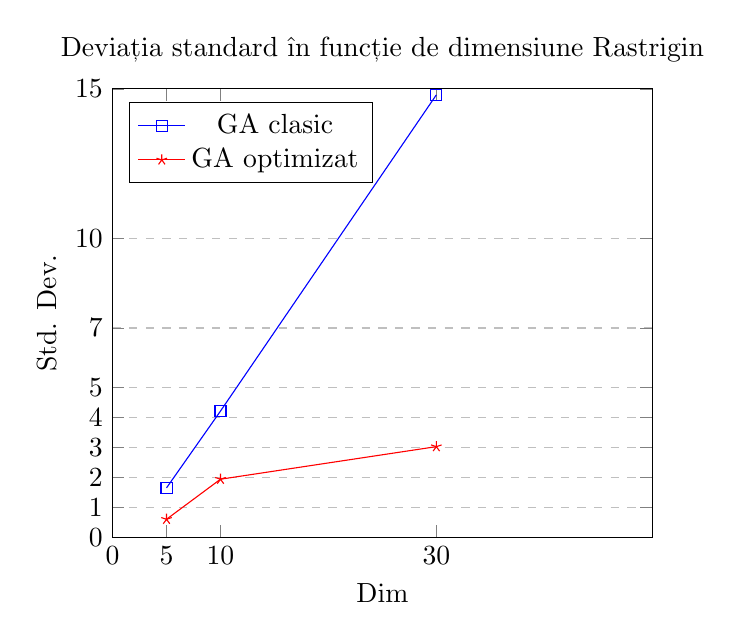
\begin{tikzpicture}
\begin{axis}[
    title={Deviația standard în funcție de dimensiune Rastrigin},
    xlabel={Dim},
    ylabel={Std. Dev.},
    xmin=0, xmax=50,
    ymin=0, ymax=15,
    xtick={0, 5, 10, 30},
    ytick={0, 1, 2, 3, 4, 5, 7, 10, 15},
    legend pos=north west,
    ymajorgrids=true,
    grid style=dashed,
]

\addplot[
    color=blue,
    mark=square,
    ]
    coordinates {
    (5,1.65)(10,4.22)(30,14.80)
    };
 
    
\addplot[
    color=red,
    mark=star,
    ]
    coordinates {
    (5,0.60)(10,1.94)(30,3.03)
    };
    \legend{GA clasic, GA optimizat}
    
    
\end{axis}
\end{tikzpicture}

\section{Concluzii}
Varianta optimizată a algoritmului genetic oferă soluții mai bune decât cea simpla pe primele 3 funcții de test (Rastrigin, DeJong1 și Michalewicz) și oferă soluții apropiate de cele ale metodelor BIHC, FIHC și SA, uneori chiar mai bune. În cazul funcției lui DeJong1 se gasește chiar rezultatul exact pe toate cele 3 dimensiuni.\\
Cea mai mare îmbunătățire (fața de varianta clasică) se observa pe funcția lui Rastrigin de dimensiune 30 (de la o medie de 84.42 la una de 45.62). Tot pe această funcție se observă o scadere accentuată a deviației standard.\\
În cazul funcției lui Schwefel toate rezultatele sunt mai slabe decât la varianta clasică a GA iar timpul este și el mult mai mare. În cazul Schwefel pe 30 dimensiuni eroarea este chiar uriașă.


\begin{thebibliography}{9}

\bibitem{Maxim și minim}
  Minim și maxim\\
  \url{https://en.wikipedia.org/wiki/Maxima_and_minima}
  
\bibitem{Intocmirea raportului}
  \begin{flushleft}
  Intocmirea unui raport \\ Formularea introducerii.
  \url{https://www.monash.edu/rlo/assignment-samples/engineering/eng-writing-technical-reports/introduction}
  \end{flushleft}
\bibitem{Algoritm genetic}
  Algoritm genetic\\
  \url{https://www.geeksforgeeks.org/genetic-algorithms/}\\
  \url{http://www.lendek.net/teaching/opt_en/ga.pdf}\\
    \url{https://profs.info.uaic.ro/~eugennc/teaching/ga/}\\
\bibitem{Codificare Gray}
  Codificare Gray\\
  \url{https://www.geeksforgeeks.org/gray-to-binary-and-binary-to-gray-conversion/}
  
 \bibitem{De Jong1}
  De Jong1\\
  \url{http://www.geatbx.com/docu/fcnindex-01.html#P89_3085}\\
  Grafic\\
\url{https://www.sfu.ca/~ssurjano/spheref.html}
  
\bibitem{Schwefel}
  Schwefel\\
  \url{http://www.geatbx.com/docu/fcnindex-01.html#P150_6749}\\
    Grafic\\
\url{https://www.sfu.ca/~ssurjano/schwef.html}
  
\bibitem{Rastrigin}
  Rastrigin\\
  \url{http://www.geatbx.com/docu/fcnindex-01.html#P140_6155}\\
    Grafic\\
\url{https://www.sfu.ca/~ssurjano/rastr.html}
  
\bibitem{Michalewicz}
  Michalewicz\\
  \url{http://www.geatbx.com/docu/fcnindex-01.html#P204_10395}\\
  \url{http://www.alliot.mobi/papers/gecco2014b.pdf}\\
    Grafic\\
\url{https://www.sfu.ca/~ssurjano/michal.html}
  
  
\end{thebibliography}  
\end{document}